% ------------------------------------------------------------------------ %
% !TEX encoding = UTF-8 Unicode
% !TEX TS-program = pdflatex
% !TEX root = ../Tesi.tex
% !TEX spellcheck = it-IT
% ------------------------------------------------------------------------ %
%
% ------------------------------------------------------------------------ %
% 	STATO DELL'ARTE
% ------------------------------------------------------------------------ %
%
\chapter[Occupancy Monitoring and State of the Art]{Occupancy Monitoring Basics and State of the Art}
%
%\markboth{x}{y}	% headings
%
\label{cap:soa}
%
%cosa sono gli smart buildings e perchè è importante l'occupancy monitoiring

Smart buildings are environments like offices or schools able to exploit sensors, devices and appliances to observe users activity and adapt autonomously taking decisions to achieve comfort, safety and energy efficiency. Considering the fast development of technologies for connected sensor and actuator (the so called \emph{Internet of Things}), since few years smart buildings are becoming a reality from a technological point of view.

Both the industry and the academia have put a lot of effort in the research of smart buildings. In some commercial products the term \emph{smart} is often referred to devices that can be remotely accessed and managed, even though there is no intelligence involved. In this thesis the term \emph{smart building} refers to the concept of environment able to cooperate and self-organize its components observing the indoor space.

\medskip
One of the main components of a smart building is the \textbf{Occupancy Monitoring system}, i.e. a system able to detect the number (or even the identity) of the occupants in every room or zone of the building. Occupants play a key role in the objectives of smart buildings. User comfort can be improved controlling automatically the environment temperature, humidity, and brightness, setting all the parameters exploiting user defined preferences. In this scenario, user identification and localization inside the building is fundamental. 

\smallskip
In order to guarantee the building safety, the knowledge of the occupants position in real-time can be precious. In case of emergencies like fires, escape routes and emergency exits might be highlighted with notifications targeted to the specific user's location \cite{Piscitello2015}. Rescue operations can be organized faster and more efficiently when the position of injured occupants is known. Complex safety systems are even able to automatically detect dangerous situations like terrorist attacks when fast mass-movement of people happen from a room to another.

\smallskip
Probably, the main purpose of smart buildings, or in this case also called green buildings, is energy sustainability.
In the last few years, plenty of methods have been proposed to learn the building occupants habits and to use such information to forecast the energy consumption.
Many of these approach are based on the concept of \emph{Smart Grid}. Smart Grid is a traditional electric grid enhanced with a two-way communication between the provider and its customers to respond digitally and more efficiently at quickly changing electric demand.
The mentioned methods for smart buildings are able to select the most appropriate appliance usage scheduling given a energy reduction request coming from the smart grid. Also in this case an occupancy monitoring system is essential to recognize users activities.

\medskip
The expected outcome of an occupancy monitoring system is the detection in real-time (or with a tolerable delay) of every user inside the building, with their position. Usually, the occupant needs to be localized in a zone or room of the building, since this information is sufficient to automatize HVAC and lighting systems. In cases of automation based on user-defined preferences also the identification of each user is required by the system.
At first look, the occupancy monitoring problem can be associated at the more traditional problem of the indoor localization. Even though the two problem share some characteristics, we will see that conventional solution for indoor localization are not directly applicable for monitoring (section \ref{subsec:wips_od}).

\smallskip
As we will see in this chapter, a lot of effort has been put both from the industry and the academia in terms of research and product industrialization. However, some intrinsically hard challenges of the occupancy monitoring problem bring to the lack of an accessible solution with broad adoption.

%il problema sembra simile o identico al più tradizionale indoor localization. non è così perchè ....
%come vedremo i due problemi sono simili ma le classiche soluzioni di WIPS non sono direttamente applicabili per O.M.

% ------------------------------------------------------------------------ %
\section{Evaluation Metrics}
% The traditional concept of indoor localization is a service able to assist the user during orientation in an unknown space, and to assist the navigation from one point to another. in this scenario, the end-user is the main subject who benefits from the positioning information.\\
% With the diffusion of smart spaces that cleverly support their inhabitants, positioning information is becoming essential also on the infrastructure side, usually called Building Management System (BMS).

Occupancy Monitoring systems have the purpose to detect the number of occupants in a building, their position and in some cases also the identity of each one.
Occupancy detection solutions can range to deeply different implementations, depending on the technologies exploited to detect human presence. In this section will be defined some metrics and aspects of occupancy monitoring systems useful to evaluate and compare different solutions.

\medskip
A feature that characterizes different occupancy monitoring systems is \textbf{Resolution} (Fig~\ref{fig:resolution}): it represents the granularity of the measurement.

\begin{figure*}
\center

\minipage{0.51\textwidth}
  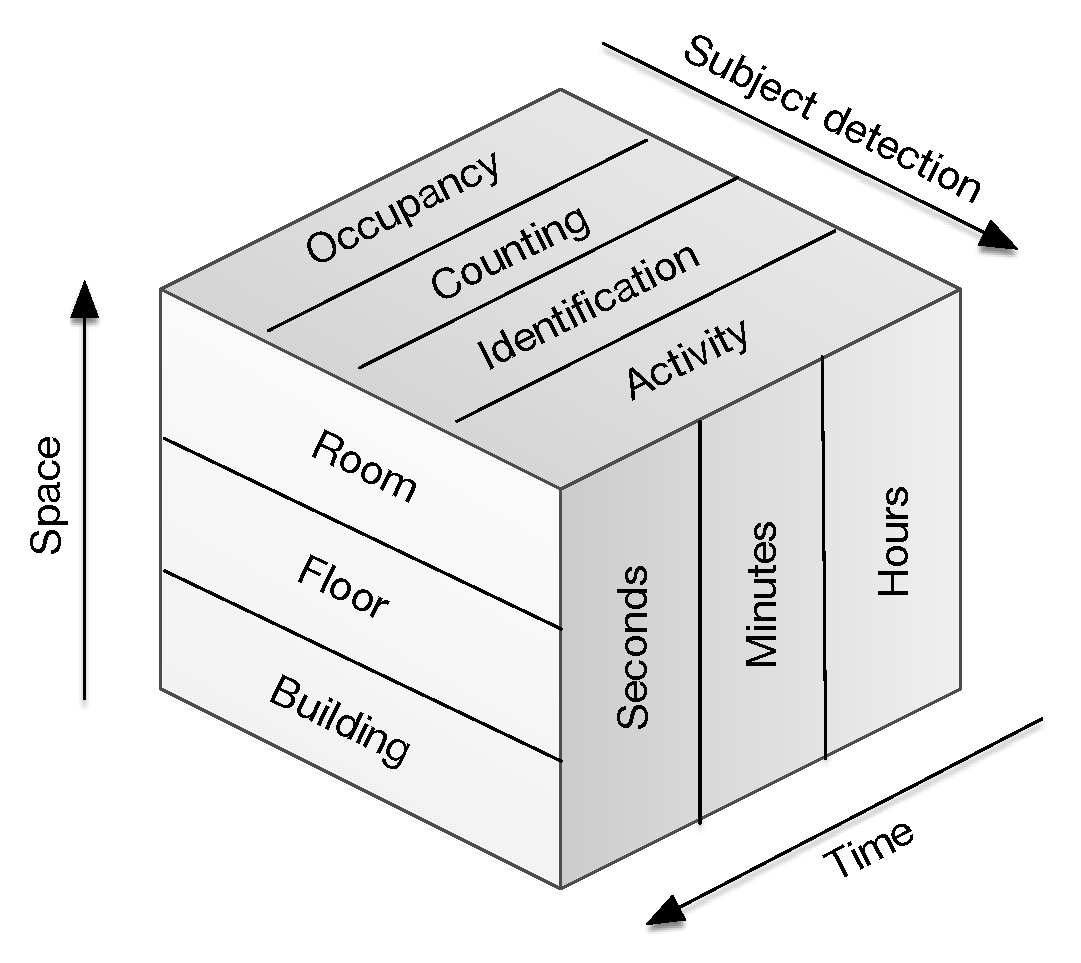
\includegraphics[width=\linewidth]{resolution.pdf}
  \caption{Occupancy Monitoring systems resolution.}\label{fig:resolution}
\endminipage\hfill
\minipage{0.49\textwidth}%
  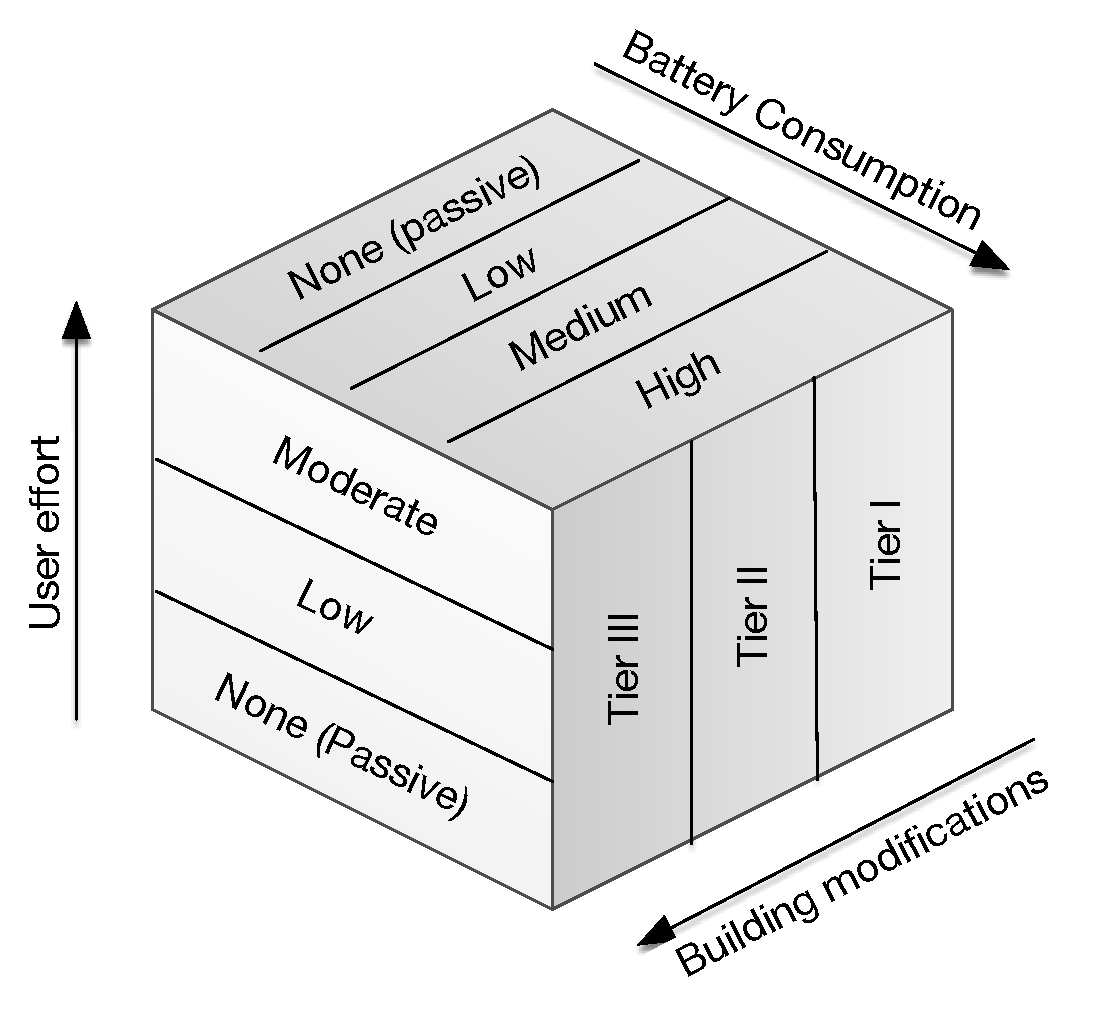
\includegraphics[width=\linewidth]{intrusiveness.pdf}
  \caption{Occupancy Monitoring systems intrusiveness.}\label{fig:intrusiveness}
\endminipage
\end{figure*}

Resolution can refer to:
\begin{itemize}
\item Subject of the detection: from low to high resolution, the system can perceive only the occupied/unoccupied status of a zone, the number of people or even the identity of each person.
\item Space resolution, i.e. the smallest region in which the user can be localized. Can range from building zones to single rooms, desktop stations or cubicles.
%In this terms, occupancy monitoring usually requires lower levels of resolution than localization.
\item Temporal resolution indicates the smallest time span in which occupancy status transitions can be reported. For real-time applications, small delays are always required to avoid user waits and annoyances.
\end{itemize}

\medskip
A common metric to valuate and compare any solution is the \textbf{Accuracy} of the system, an index that describe how much the resulting measurement differs from the true value (also called \emph{Ground Truth}). In our context, detection accuracy is the capability to correctly recognize occupied/unoccupied state of the rooms; occupancy estimation accuracy reveals how much the number of estimated people in the room differs from the actual number of occupants. A good level of accuracy is essential for almost every detection systems: as instance, in order to reach energy waste reduction, false positive presence detections can be counterproductive since appliances would be turned-on in empty rooms.

\medskip
Accuracy and resolution are good parameters to summarize the system performances, but are not sufficient to describe how much the solution is desirable and attractive for real commercial applications. For instance, approaches that provide high accuracy and resolution tend to have also a higher \textbf{Cost}, complex \textbf{Installations} and higher \textbf{intrusiveness} for the occupants (see Fig.~\ref{fig:intrusiveness}). To classify installation complexity, three levels, or \emph{tiers}, have been identified by  Akkaya et al. \cite{Akkaya2015}:

\begin{itemize}
  \item Tier \rom{1} requires no modifications to the existing systems other than a data collection and processing unit. Solutions at this level make use of already existing building infrastructures, such as local network or electricity meters to measure occupancy. This approach is called \emph{implicit} occupancy sensing, and will be discussed in section \ref{subsec:implicit}.
  \item Tier \rom{2} is characterized by fast software and/or hardware installations to make occupancy related data available. Training phases are fast or immediate to execute, and can be accomplished by one or few building administrators.
  \item Tier \rom{3} involves the addition of software and hardware that requires complex installations or long training periods. Complex installations include precise measurements of the building geometry in order to know the exact position of every installed device. Long training periods are usually required by solutions that extract occupancy information from ambient data (see section \ref{subsec:ambient}).
\end{itemize}

Usually higher tiers also imply higher costs for hardware purchase, system maintenance and computational resources. For occupancy monitoring systems, keeping low the installation and running costs is crucial, since spending cut is one of the main purposes of building renovations.

Another factor that need to be considered to promote the adoption of a monitoring system is the \textbf{Intrusiveness} on the users routine. Intrusiveness describe how much the user activity is negatively affected by the system.
%Since localization systems used for orientation and navigation are executed for a limited amount of time (typically in the order of minutes), indoor localization techniques doesn't take into consideration the system intrusiveness caused, for example, by high levels of power consumption.
In occupancy monitoring systems, where positioning data needs to be continuously collected during many hours of the day, a low level of system intrusiveness is essential.
Implicit occupancy sensing (tier \rom{1}) is usually completely passive and doesn't require the occupant to use any additional device or software.
Other solutions instead, relies on the assumption that the occupants are always accompanied by a tag, a smartphone or a wearable device. This can be quantified more or less by a "low effort" required to the user. This amount of effort can be perceived differently depending on the situations. At work for example, where the user is used to guarantee phone call and email availability, the effort can be nearly zero; at home instead, where some users are used to empty their pockets as soon as they are inside, the effort can be high.
However, for solutions based on smart devices, the aspect that more affects users routine is the battery consumption. Smart devices are becoming omnipresent around people and they can be considered as an extension of ourselves. A possible weak point of every smart device is the battery life, that becomes an issue also for the user daily activity. For this reasons, occupancy detection systems that rely on smart devices should carefully consider the energy efficiency of the device. A system that cause a considerable increase in battery drain directly afflict the user comfort and peace of mind, and can bring the user to leave the application. Nevertheless, we'll see in the next sections that many wireless based solutions present in literature that exploit smart devices completely ignore the energy problem.

System intrusiveness, from both the points of view of the building equipment and the user activity, is summarized in figure \ref{fig:intrusiveness}.

% In conclusion, the main differences between traditional indoor localization and monitoring systems like BlueSentinel are (Fig.~\ref{fig:locvsmon}):
% \begin{itemize}
% \item Resolution of the measurement, where localization usually gives more resolute estimation;
% \item Duration of execution is usually very short for navigation and orientation tasks, while can last for many hours in occupancy monitoring;
% \item Battery consumption (per time unit) is not an issue during brief orientation, while in occupancy monitoring must be very low to guarantee several hours of execution.
% \end{itemize}

\section{Existing Solutions}
\label{sec:soa}
In this section are reviewed some of the most relevant approaches proposed in literature to solve the occupancy monitoring problem, grouped by their respective enabling technologies. A particular attention is directed to wireless-based indoor positioning systems (section \ref{sec:wips}), how they have been exploited for occupancy monitoring and their limitations in this specific context.

\subsection{Traditional solutions}
The traditional solutions used to face the occupancy detection problem are based on passive infrared sensors (PIR), door badges or radio frequency identification tags (RFID tags). PIR sensors are used to detect people movements in order to control lighting, doors and other appliances.
The main issue is that overly still occupants become invisible to these sensors. In some cases, door sensors have been added to mitigate this issue. How will be explained in section \ref{subsec:ambient}, usually PIR are used in combination with other ambient sensors because of their low accuracy and their inability to provide estimations on the number of occupants.

In RFID systems, antennas are displaced inside the building to detect the presence of tags co-located with the occupants. However, few RFID systems can reach 10 meters of working range increasing the number of minimum antenna; in addition, tag transmissions are easily disrupted by other radio-frequency sources.

% TODO: research info RFID in traditional solutions

\subsection{Implicit Sensing Solutions}
\label{subsec:implicit}
Implicit occupancy sensing is the use of existing building infrastructure (that is not originally intended for occupancy detection) to measure occupancy. Implicit sensing relies on the notion that the effects passively produced by occupants on building systems can be used to determine occupancy information.

\smallskip
An example is those proposed by Melfi et al. in \cite{Melfi2011} that measures occupancy using existing network infrastructure: their method consists in the collection of MAC and IP addresses in routers that are successively correlated to the occupancy of a building, a zone, and/or a room. The main idea is that when a client sends a WiFi packet to an Access Point (AP), it is assumed to be located within the range of the AP.
They collect data from Address Resolution Protocol tables (or ARP cache) and Dynamic Host Control Protocol (DHCP), of available access points, and derive the occupancy level of each area.
The approach reveals a low occupancy accuracy (59\%), caused by two main problems. First the overlap of AP coverage results in devices connecting to APs that are not the nearest available. Second, the inconsistence of mobile devices that lose connectivity causing false negatives.\\
Although they obtained low levels of occupancy accuracy with respect to the ground truth, they proposed one the first solutions able to re-use infrastructures common to many (if not most) building types, and does not require any additional hardware or physical modification.

\smallskip
Balaji et al. proposed Sentinel \cite{Balaji2013}, another WiFi based occupancy detection system used to actuate on HVAC. They used the protected network of the University of California (San Diego) to collects packets coming from users' devices and infer occupancy. Also in this work, clients location has been assumed to be in the range of the receiving AP. In order to increase accuracy, building zones have been divided into personal spaces, with the constraint that a personal space cannot be occupied unless the owner is present in the space. This approach is represented in figure \ref{fig:sentinel}. If the AP does not hear from the client for a fixed period of time (1000 seconds in their network), the connection is terminated and the user is considered out of the zone.

\begin{figure}[h!tb]
\centering
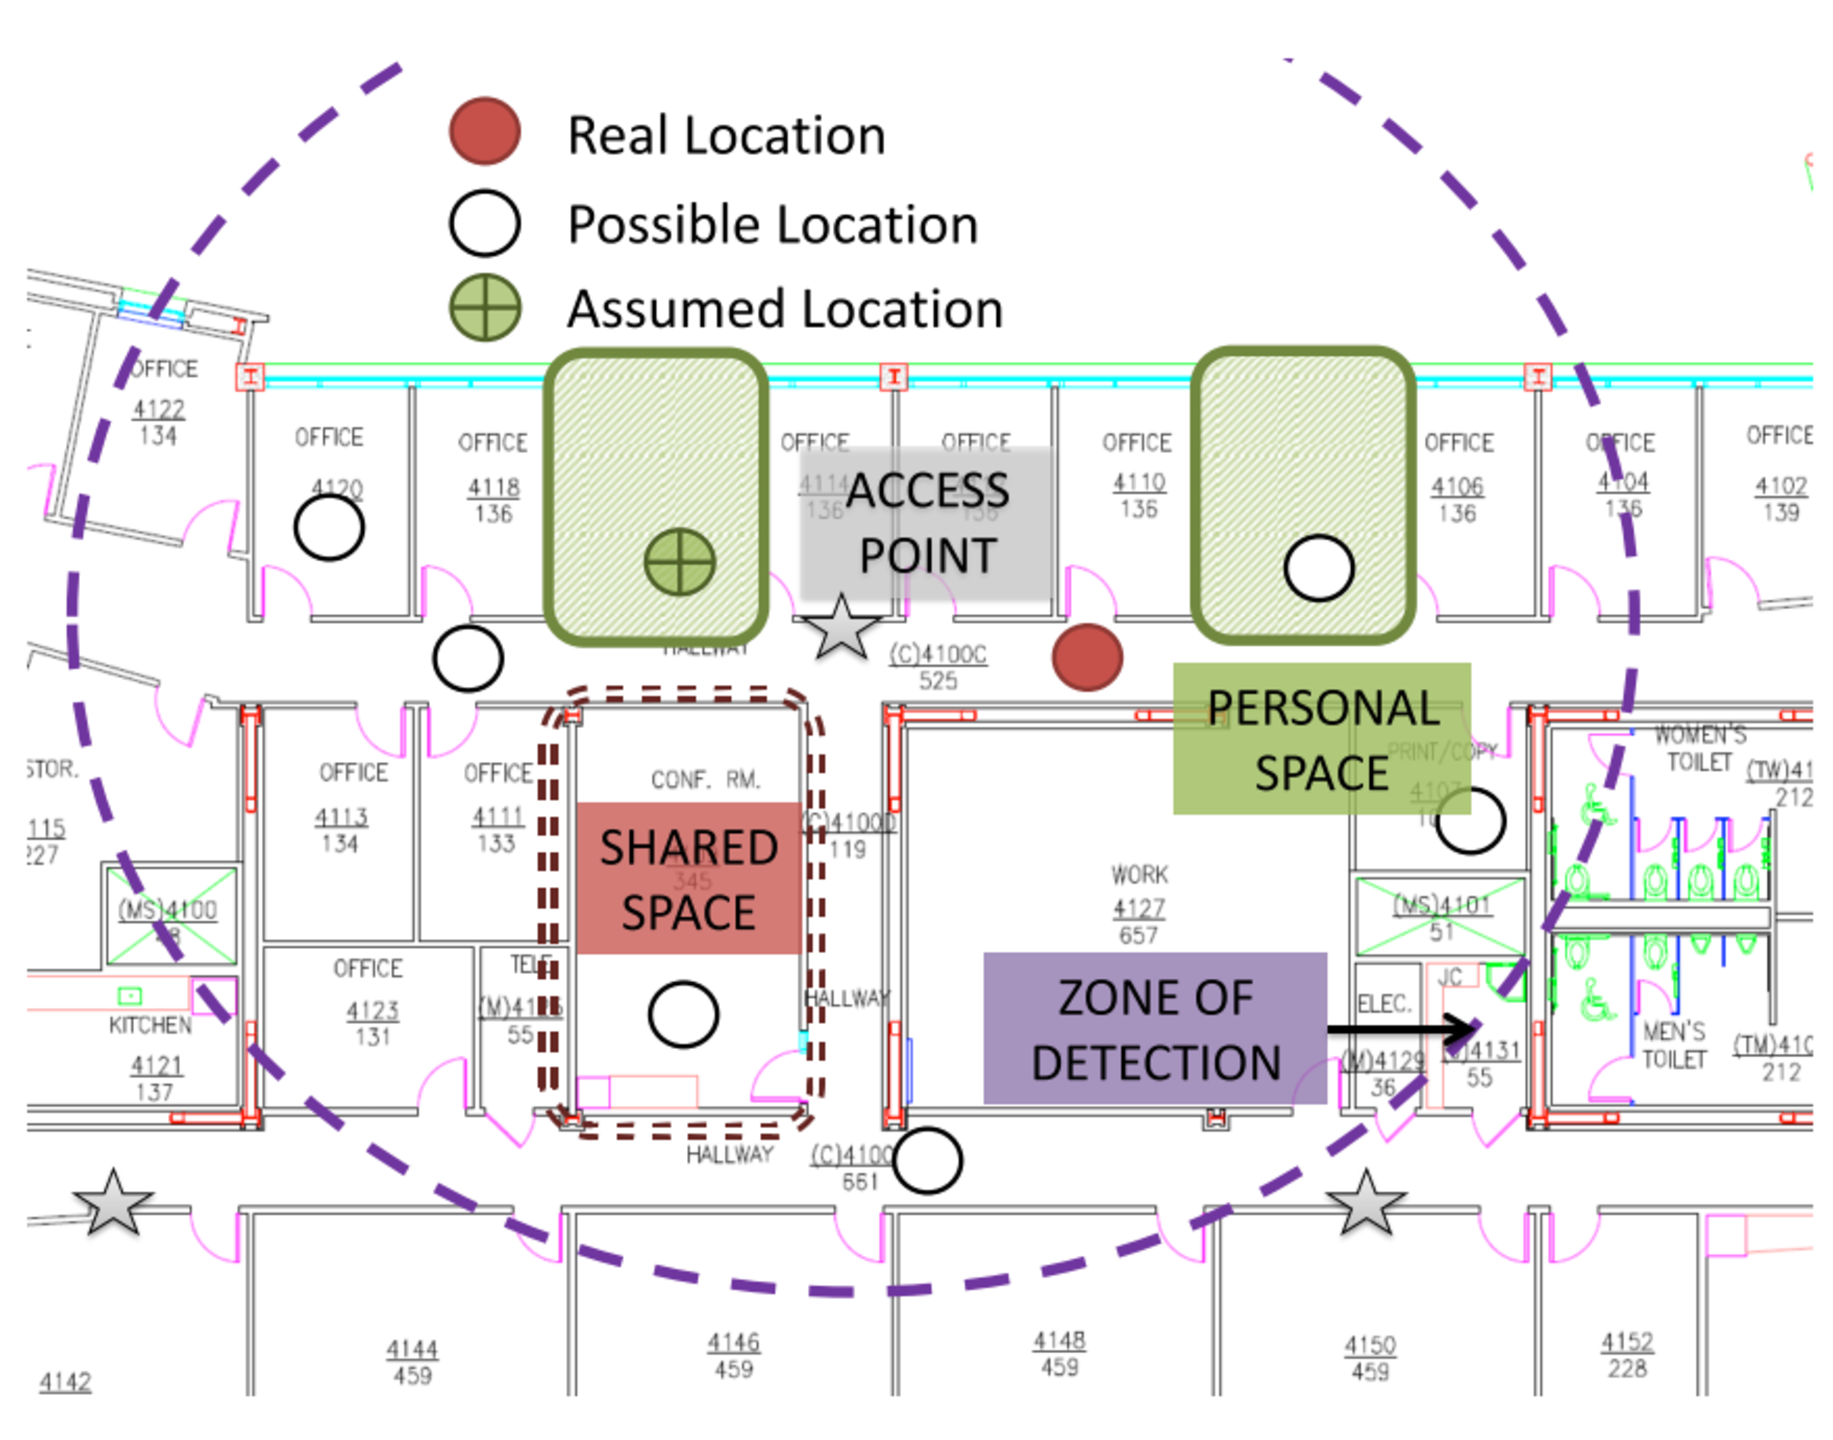
\includegraphics[width=0.6\linewidth]{sentinel.pdf}
\caption[Occupancy inference of the Sentinel system using WiFi connectivity]{Occupancy inference of the Sentinel system using WiFi connectivity. The occupant is assumed to be in her personal space whenever she is within the associated AP’s zone of detection, as denoted by “Assumed Location”.}
\label{fig:sentinel}
\end{figure}

Since an occupant can have different WiFi devices, Balaji et al. decided to use the smartphone as the most representative of the user position. However, the algorithm that they implemented in order to distinguish the phone from the others devices in APs logs has a high level of inaccuracy, causing a degradation of overall results. In addition, smartphones revealed an aggressive sleep policy on WiFi activity as soon as the screen is locked, determining lack of packets and significant false negative detections of occupancy.

\medskip
Implicit sensing solutions have very low costs of installation and don't require the user to do anything except their usual activity. Implicit sensing is usually characterized by low levels of accuracy and resolution; for example can be difficult, if not impossible, to distinguish if more than one connected devices belong to a single occupant of the building. Due to the low performances, implicit sensing is not a suitable source of information for real-time applications like appliance control or safety operations, but thanks to the easy and inexpensive implementation can be always used to collect historical data and to extract long-term occupancy probabilities as a function of time.

\subsection{Ambient Sensor Networks}
\label{subsec:ambient}
Thanks to the diffusion of low cost and low power sensors, and the emerging research area on Wireless Sensor Networks (WSN), solutions based on ambient sensing are currently deeply investigated.
The basic idea is that human presence inside the building continuously affects ambient factors like temperature, humidity, sound, CO\(_2\) and so on. By monitoring these factors the system can estimate the number of occupants.
At this purpose, sensor motes are applied to each room of the building; data is sent to a centralized system where an algorithm estimates the number of occupants. One of the main issues of this approach is the long training period required to build the model, causing time consuming and intrusive data collection. We report two works that tried to overcome this issue.

\smallskip
Beltran et al. proposed ThermoSense \cite{Beltran2013}, a wireless sensor network of nodes that can measure occupancy of rooms. Each node implements a combination of thermal sensor array and PIR sensor. Since occupants are typically warmer than the surroundings, the thermal sensor array, that is capable of measuring multiple temperatures with an area, is used for detecting occupancy. For distinguish between people from passive warm objects, the PIR functionality is exploited. If the PIR sensor indicates the room is empty, then the array determines the thermal background of the space, otherwise the system tries to recognize the number of hotspot corresponding to occupants.\\
The thermal sensor array used is able to measure temperatures in an 8x8 grid pattern within an 2.5mx2.5m area, when placed at a height of 3m (ceiling). A photo of the employed sensor mote and the resulting detection is reported in figure \ref{fig:thermosense}. The system was able to measure occupancy with a Root Mean Square Error of 0.35 person. The weak point of this implementation relies on the short coverage of single sensors, that heavily increases the cost of installation. In order to fully cover a simple 10mx10m room, 16 nodes would be necessary. Covering only hot points like desktop stations or cubicles would drastically reduce the accuracy.

\begin{figure*}
\center
\minipage{0.5\textwidth}
  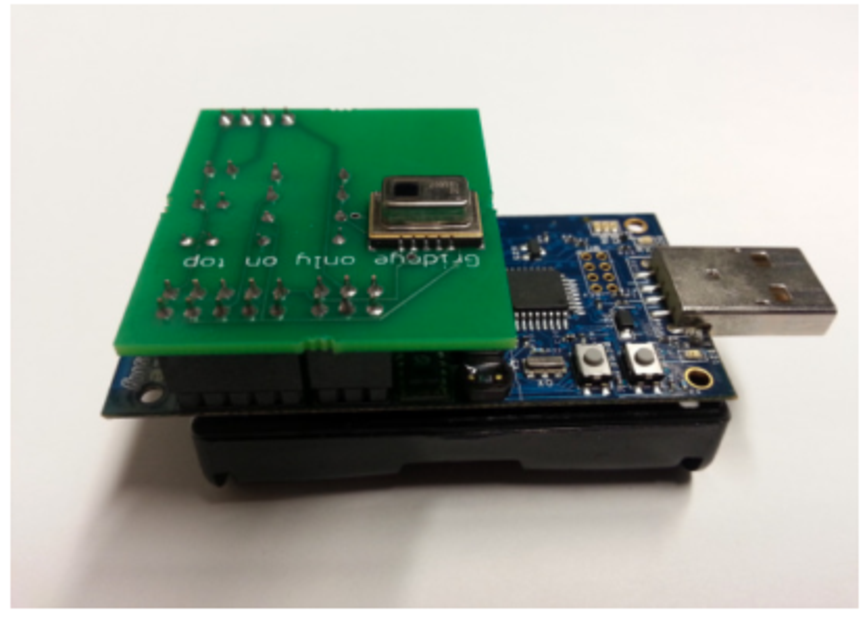
\includegraphics[width=\linewidth]{thermosense1.pdf}
\endminipage\hfill
\minipage{0.5\textwidth}
\center
  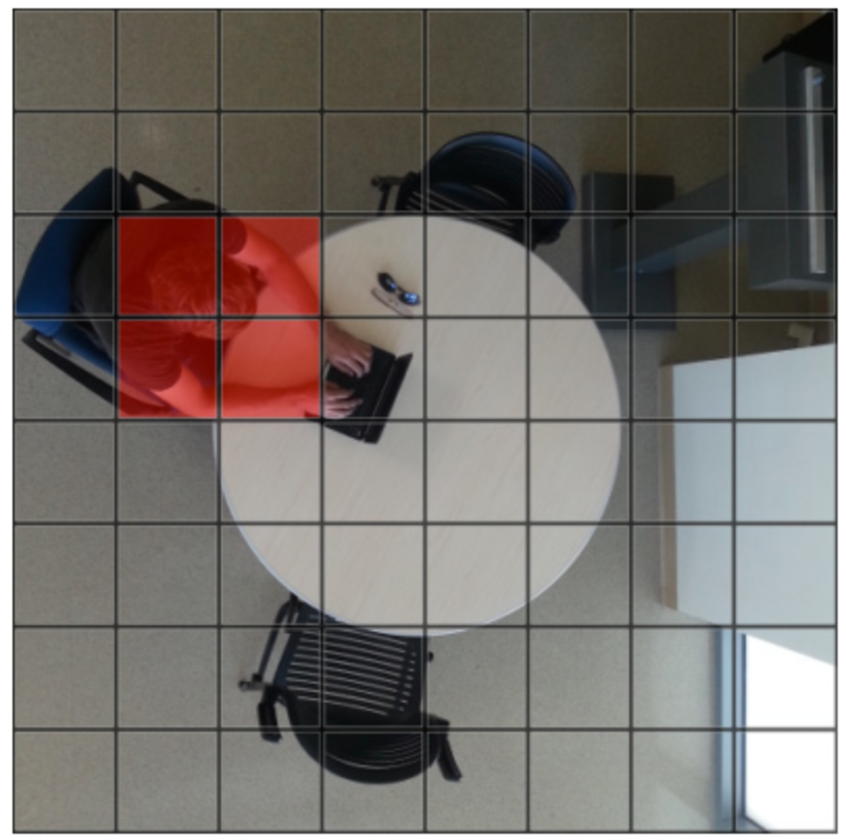
\includegraphics[width=0.8\linewidth]{thermosense2.pdf}
\endminipage
\caption{Thermal sensor array employed in the Thermosense system and its occupancy detection outcome.}\label{fig:thermosense}
\end{figure*}

\smallskip
Zheng et al. \cite{Cossio2012} proposed a framework for cross-space occupancy modeling in which the model is trained in a space only a single time, and then applied to other geometrically similar spaces. The objective of their study was to generalize relationships between occupancy and ambient factors, collected through sensor boxes equipped with several different sensors: light, sound, motion, CO2, temperature, humidity, PIR and door switch. Training data has been collected from six rooms for long periods of time (10 / 18 months). The occupancy ground truth was collected using ceiling-mounted cameras, which captured images every 10 seconds. Occupancy was then manually labeled for the ground truth. After a phase of selection and pre-processing, the ambient features were used by five supervised learning classifiers to build the general model.\\
The occupancy model was then tested applying samples from other geometrically similar rooms. The modeled occupancy was compared with the actual occupancy detection from 6:00 AM to 9:00 PM (only weekdays) to calculate the performance. They experienced a daily F-measure from \numrange{0.71}{0.94} and a daily RMSE from \numrange{0.42}{1.72} person. However, training rooms employed accommodate no more than four occupants, suggesting that the performances of such model could drastically drop if applied to more populated areas.

\medskip
The advantage of similar solutions is that the user is not forced to keep devices with him/her to be detected by the system. Intrusiveness on the occupant is rather low, except for the employment of cameras and microphones that strongly reduce the privacy.\\
The principal issue of ambient sensing solutions is that ambient factors variate slowly, and provide fast reactions to users movements is difficult. Second, ambient models requires long training period in order to teach the algorithm the relationships between occupancy and ambient factors.
Other complications arise because ambient factors are influenced, besides occupancy, also by HVAC and lighting systems. HVAC and lighting are often the appliances that occupancy detection outputs should regulate, creating undesired feedbacks in the control system.

\subsection{Cameras}
\label{subsec:cameras}
Cameras can be used for measuring occupancy exploiting image analysis algorithms, that recognize bodies or faces within captured images.

\smallskip
Erickson et al. developed OPTNet \cite{Erickson2013}, an occupancy estimation system comprised of 22 node wireless camera nodes used as an optical turnstile to measure area/zone occupancies. They employed a lightweight on-board image processing algorithm along with classification techniques in order to detect occupants' transitions. In addition, they exploited a 40 node PIR wireless sensor network to improve the system accuracy. Figure \ref{fig:optnet} reports two photos of the deployed camera systems and an example of image analyzed. Their work claims to be capable of detecting occupants transitions with up to 94\% accuracy and that the overall system was able to bound the error of occupancy within 1.83 people on average for their building.

\begin{figure}[h!tb]
\centering
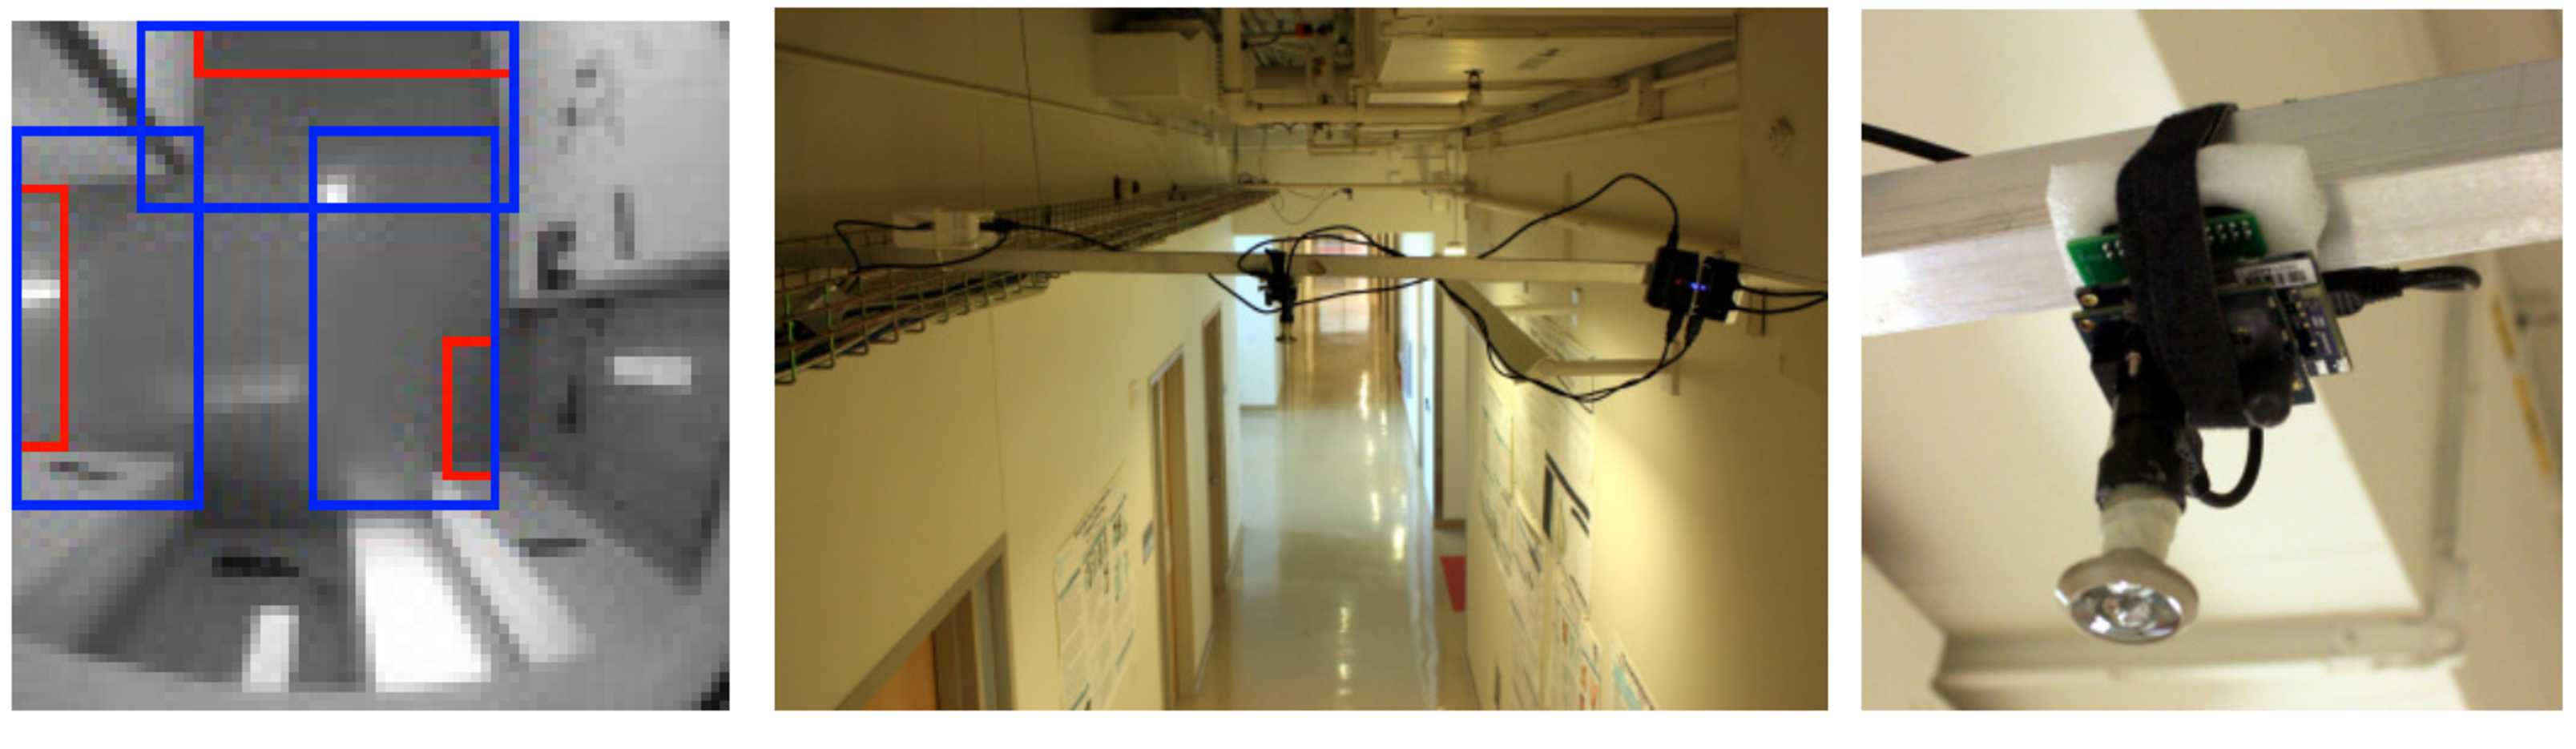
\includegraphics[width=\linewidth]{optnet.pdf}
\caption[The deployed OPTNet system.]{The deployed OPTNet system. Transition areas are represented as bigger blue boxes while trigger areas are small red boxes.}
\label{fig:optnet}
\end{figure}

\medskip
Camera placement is a considerable issue. Cameras placed in offices or meeting rooms raise privacy concerns. A flexible solution for different privacy requirements (and legislations) should allow to keep track of anonymous occupants without collects sensitive data like faces pictures. Cameras can be placed in public and narrow transition points, like hallways or stairways and function as an "optical" turnstile, counting people for each direction. This strategy however is prone to cumulative error: If an optical turnstile misses even a single person entering/exiting a space, this error is propagated until another offsetting error occurs or some other mechanism is used to remove the cumulative error. To give an example, if the last person in an office leaves at 7 p.m. and this transition is missed, then the space will continue to be erroneously considered occupied.\\
Another problem of camera based systems is the computational effort required by the image analysis algorithms. One of the main purpose of smart buildings is the reduction of costs through energy harvesting. In this perspective, the installation of expensive hardware with high computational resources and consumptions for image processing is not the most appealing solution.

\section{Wireless Indoor Positioning}
\label{sec:wips}

In order to determine the position of a user (or an object) in a limited physical space, positioning systems based on wireless technologies have been studied and employed from many years.
Wireless positioning systems, even with deeply different implementation technologies, always rely on a set of reference nodes that communicates with the target object to be localized through generic radio frequency signals.
GPS as instance, the well-known Global Positioning Systems, is able to provides location information anywhere on the Earth where there is an unobstructed line-of-sight with at least four GPS satellites. GPS, which is able to provide good performance levels in open spaces, has been widely adopted for outdoor applications; however, is not capable of operating indoors, due to the significant attenuation introduced by buildings walls and ceilings.

\smallskip
During last years, solutions for indoor localization have been proposed; in this case reference points are represented by WiFi access points or beacons enabled with different signal protocols like Bluetooth.
Some existing solutions that exploit WiFi infrastructure have already been discussed in section \ref{subsec:implicit}. In that case however, the location estimation was performed based on access points data like MAC or IP addresses collected at the Network layer of the OSI model. In this section instead will be discussed localization techniques that analyze the wireless signals at a lower level (Physical OSI layer). For this reason, this section provides first some background concepts of radio signals, later an overview of the most common localization techniques based on signal analysis and finally some relevant related works.

\subsection{Signal Transmission}
\label{subsec:sig_tx}
Electromagnetic signals are classified according to their frequency. Radio frequency (RF) includes all the wave frequencies that lie in the range extending from around 3 kHz to 300 GHz, which include those frequencies used for the most common wireless communications. For this reason the term \emph{Radio Frequency} (or its abbreviation RF) is used as a synonym for radio, describing the use of wireless communication as opposed to communication via electric wires.

The signal transmitted by an antenna can be expressed as a function of time:


\begin{equation}\label{eq:sig_func}
s(t) = a(t) \cos [2 \pi f_c t + \theta(t)]
\end{equation}

where $\theta(t)$ is the phase, $f_c$ is the carrier frequency. A useful measurement of radio signals is power, or more precisely the average power, defined as the time average of energy:

\begin{equation}\label{eq:sig_power}
P = \lim_{T \to +\infty} \frac{1}{2T} \int\limits_{-T}^{+T} (|s(t)|)^2 dt
\end{equation}

When an antenna transmits a RF signal, the signal is characterized by a certain power. The signal at this point is transformed by the antenna into a electromagnetic wave. During propagation the signal travels a medium that introduces some power attenuation to the signal. When the signal hits the receiving antenna this attenuation, also called \emph{Path Loss}, can be expressed as:

\begin{equation}\label{eq:path_loss}
PL = \frac{P_t}{P_r}
\end{equation}

where $P_t$ is the power of the transmitted signal while $P_r$ refers to receiving signal. Different transmission mediums, like free space, air, walls or bodies, can introduce different attenuations. In free space the attenuation is minimal and is in fact called free-space loss. In other materials additional attenuation is introduced by effects like refraction, diffraction, reflection, and absorption. If the medium is completely composed by the free space or the air, the transmission link is referred as Line of Sight (LOS). Differently, if the signal needs to travel across other materials in order to reach the receiving antenna, the communication is called Non Line of Sight (NLOS).

Usually the path loss is expressed in decibels (dB):

\begin{equation}\label{eq:path_loss_db}
PL_{db} = 10\log_{10}(\frac{P_t}{P_r})
\end{equation}

dB unit is a shorthand way to express the ratio of two values. To express absolute values instead, in this thesis many examples and results are expressed in dBm (Decibel-milliwatt), as returned by smartphones and sensors used for the measurements.
The unit dBm denotes an absolute power level measured in decibels and referenced to 1 milliwatt (mW). Absolute power $P$ (in watts) is converted to dBm with the formula $P_{dBm} = 10 \log (\frac{P}{1 mW})$. This equation looks almost the same as that for the dB, except that the power level $P$ has been referenced to 1 mW.

The transmission medium entails, other than the power loss of the signal, also a propagation delay. In particular, the delay depends mainly on the distance to be traveled, and secondary by the wave propagation speed of the medium. For wireless communication this propagation speed tends to $3*10^{8}$, which is equal to the speed of light in vacuum.

\subsection{Signal Analysis for Localization}
\label{subsec:sig_techniques}

Radio Frequency signals transmitted by reference nodes can be analyzed in order to compute or estimate the position of a target object or subject. Different signal characteristics has been measured at this purpose.

\begin{itemize}
\item \textbf{Time of Flight (ToF)}: As we previously said, the time a signal spend traveling from transmitter to receiver depends on the path length and the materials encountered. However, in most cases the main medium is the air and its propagation speed can be considered in good approximation equal to the constant speed in space. ToF technique exploits the resulting linear relationship between travel time and distance, computing distance between two points using the time delay between the transmitted waves.

There are two main approaches to compute ToF, \emph{single packet} and \emph{double packet}. The first simply requires that the reference nodes transmit a packet containing the timestamp of the transmission instant. The receiving mobile device estimates the distance between each nodes comparing the received timestamp with its time of arrival. However this approach requires a strong synchronization between the reference nodes and the target device.
When synchronization between reference and target nodes is impossible or too difficult to achieve, a double packet approach can still be used to determine ToF, as shown in figure \ref{fig:ToF}. This approach is based on the differential time difference of arrival, and eliminates time offsets between the reference and target nodes simply assuming that the path traveled by each packet is the same. Since the same time offset is added to the measured
time of one packet and subtracted from the other, the correct time of flight can be calculated without any synchronization with the equation:

\begin{equation}\label{eq:ToF}
ToF = \frac{T_{b1} - T_{a1} + T_{a2} - T_{b2}}{2} 
\end{equation}

Where $T_{a}$ and $T_{b}$ represent a timestamp measured using respectively node A and B local clocks.

\begin{figure}[h!tb]
\centering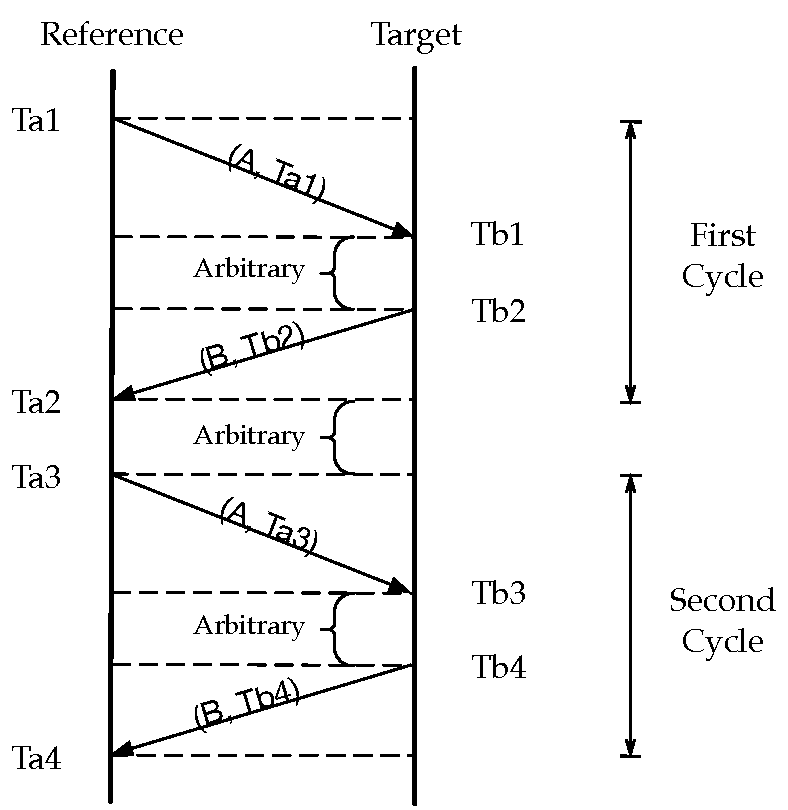
\includegraphics[scale=0.6]{ToF.pdf}
\caption{Time of Flight computation exploiting a double packet transmission.}
\label{fig:ToF}
\end{figure}

\item \textbf{Received Signal Strength Indicator (RSS or RSSI)}: is a measurement of the power present in a received radio signal. RSS can be used in two main approaches: distance estimation and fingerprinting. As introduced in \ref{subsec:sig_tx}, power loss of the signal during transmission depends on the distance, other than the medium material. The RSS perceived by a receiving node from a transmitter can be used to estimate their distance. Typically this estimation requires a prior work to be done before localization can take place. A common necessary training consists in a calibration that measures the RSS value at a fixed distance. Defining $C$ as the received signal strength collected at one meter, the run-time distance can be estimated with the following equations:

\begin{equation}\label{eq:RSS_dist}
RSS_{dBm} = -10 \alpha \log_{10}(distance) + C)
\end{equation}

\begin{equation}\label{eq:dist_RSS}
distance = 10^{\frac{(RSS - C)}{(-10 - \alpha)}}
\end{equation}

Once that three or more distances between reference and target nodes have been computed, the position can be estimated using geometric properties like trilateration.

RSS values can also be used for localization without the needs of estimating each single distance between reference and target nodes, focusing instead on the aggregate RSS information. Pattern Recognition (PR) or fingerprinting techniques attempt to engage a received power levels vector obtained from multiple reference nodes with a defined calibration test, once a time without the need for geometric algorithms. Some example of these pattern recognition techniques, that will be illustrated in the next section, are K-Nearest Neighbors (KNN), Bayesian methods, and Support Vector Machines (SVM).

Depending on OS and application, signal strength is measured either as quality in percentage, or an RSSI value in dBm. RSS values usually range from 0 (zero) to -110dBm and the closer they are to zero, the stronger the signal is. RSS level lower than -80dBm may not be usable for telecommunication, but still very useful for localization.

\item \textbf{Angle of Arrival (AoA)}: is a method for measuring the propagation direction of a RF signal incident on an antenna array. Usually AoA determines the direction by measuring the time difference of arrival at each single antenna of the array, or directly measures the angle exploiting highly directional sensors. Once that angles have been measured, position con be computed using geometric properties of triangles like in the case of RSS, but using triangulation instead of trilateration.

\end{itemize}

\subsection{Localization Techniques and Algorithms}
\label{subsec:loc_algorithms}
In the previous section there have been mentioned some properties and characteristics of wireless signals useful to infer or compute the target position. The way in which these signal properties are used to extract location encompass different algorithms and techniques. These algorithms can be classified in two main classes: \emph{Geometric} and \emph{Fingerprinting}.

Geometric algorithms are based on geometric properties of triangles. They achieve high accuracy localization, provided that the underline signal analysis is also accurate. Their biggest drawback is that they require a meticulous set-up in which distances (or angles) between the installed reference points are precisely measured in order to identify each reference at least in a Cartesian plane, if not in space. Some of the most common geometric techniques are reported below.

\begin{itemize}
\item \textbf{Trilateration}: is the process of determining absolute or relative locations of points by measurement of distances between reference and target nodes, using the geometry of circles, triangles, or spheres. Representing the space in two dimensions, when receiving a signal from a single transmitter, target device can be situated on a circumference with the reference at the center. With two transmitters there are only two positions possible: the two points where the circles around the two transmitters intersect. Adding a third transmitter enables to eliminate one of these two possibilities.
In figure \ref{fig:trilateration}, this condition is represented by a target node T localized by means of distances $d1, d2, d3$.

\begin{figure}[h!tb]
\centering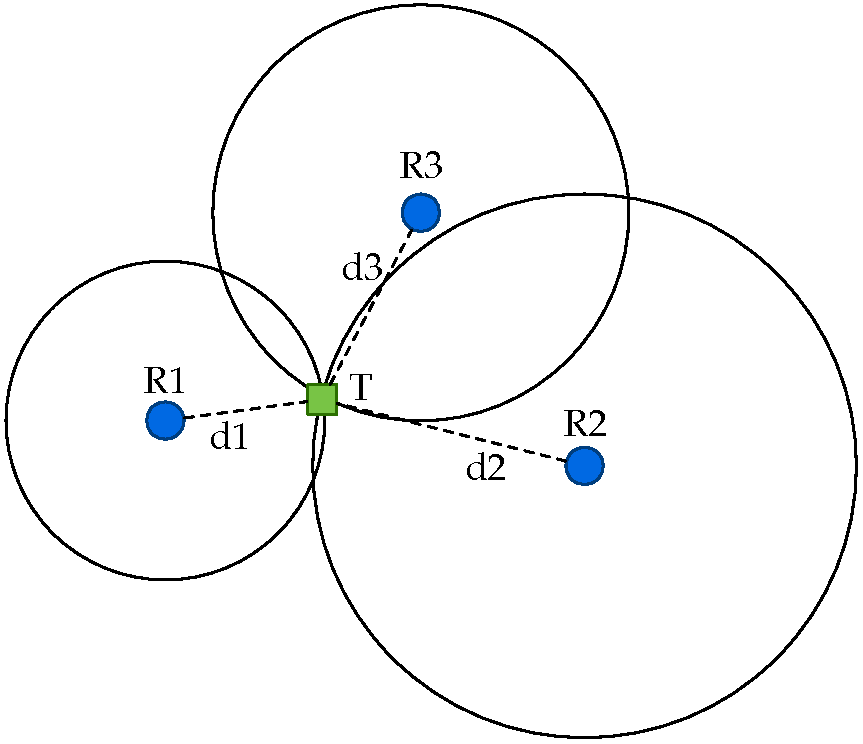
\includegraphics[scale=0.48]{trilateration.pdf}
\caption{Example of a target node $T$ localized with Trilateration by means of distances $d1, d2, d3$.}
\label{fig:trilateration}
\end{figure}

When we extend trilateration to three dimensions, the circles become spheres. In this case it's necessary to add one additional transmitter in order to find the position of the target. This explains why GPS needs to receive at least four satellites to work.

\item \textbf{Triangulation}: allows an observer (target) to calculate its position by measuring two directions towards two reference points. Since the positions of the reference points are known, it is hence possible to construct a triangle where one of the sides and two of the angles are known, with the observer at the third point. This information is enough to define the triangle completely and hence deduce the coordinates of the observer. An example of the triangle construction is reported in figure \ref{fig:triangulation} where the system is able to measure at run time $\alpha$ and $\beta$, while distance $L$ is known since the two reference points $R1$ and $R2$ have well-known coordinates.

\begin{figure}[h!tb]
\centering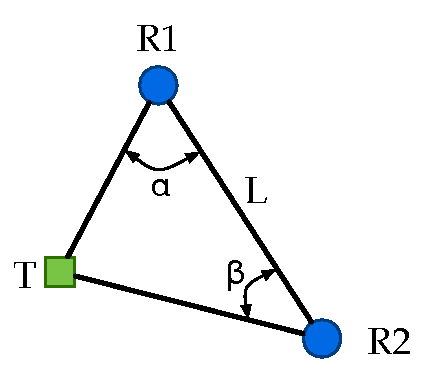
\includegraphics[scale=0.6]{triangulation.pdf}
\caption[Example of Triangulation of a target node $T$]{Example of Triangulation where the system is able to measure at run time $\alpha$ and $\beta$, while distance $L$ is known since the two reference points R1 and R2 have well-known coordinates.}
\label{fig:triangulation}
\end{figure}


\item \textbf{Min-Max algorithm}: is based on simple geometric considerations, and it is one of the most used for localization due to its easy implementation. The target node computes the distance $d_i$ from each reference node, and for each of them it draws a square with center in the position of the reference node, and edges of length $2d_i$. Then, the algorithm calculates the intersection among the squares drawn around the anchor nodes, and the mobile node is at the center of the resulting quadrilateral. In mathematical terms, the target node computes the maximum and minimum values, and it identifies a square having coordinates

\begin{equation}\label{eq:minMax}
(max_{(x_i - d_i)}, max_{(y_i - d_i)}) \times (min_{(x_i - d_i)}, min_{(y_i - d_i)})
\end{equation}

The center of this four-sided figure is the estimated position searched. An example of Min-Max estimation is shown in Figure \ref{fig:minmax}.

\begin{figure}[h!tb]
\centering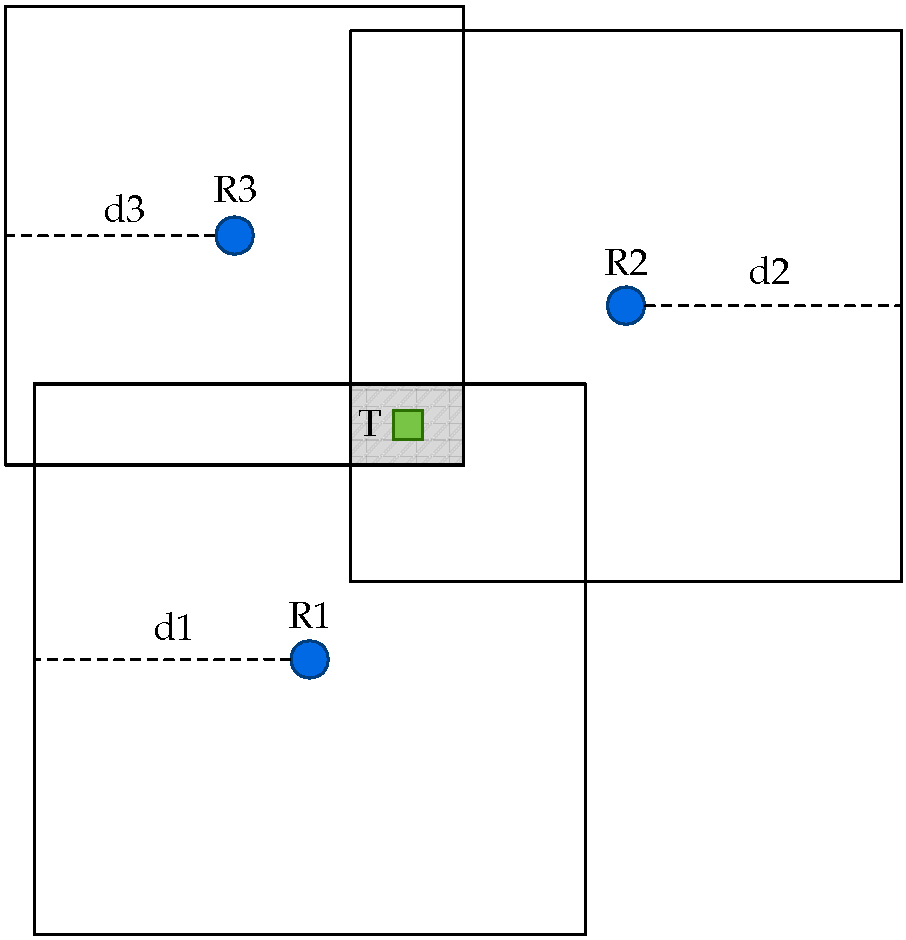
\includegraphics[scale=0.4]{minMax.pdf}
\caption[Example of MinMax computation]{Example of MinMax computation where the target node computes the distance $d_i$ from each reference node, draws a square with center in the reference node and edges of length $2d_i$. }
\label{fig:minmax}
\end{figure}

\item \textbf{Maximum Likelihood Algorithm}: is based on statistical considerations on the set of measures coming from the reference nodes. Its main aim is to minimize the Mean Square Error (MSE) of the measurements which are affected by noise. First, an estimate of distance $d_i$ to each reference device is derived from the RSSI value. Then, the node defines the error $e_i$ between the measured and the actual distance with the following equation:

\begin{equation}\label{eq:maxLike}
e_i(x_0, y_0) = d_i - \sqrt{(x_i - x_0)^2 + (y_i - y_0)^2}
\end{equation}

where $(x_0, y_0)$ is the unknown position of the target node and $(x_i,y_i)$ the position of the $i$-th reference node. To estimate the position this algorithm minimize the MSE, obtaining solutions with low error variance. Unfortunately the measurement pool need to be significant, and with only three reference nodes the accuracy can be poor.
\end{itemize}

%intro fingerprinting
Fingerprinting techniques are used to estimate the position of a mobile device based on measured signal characteristics without the constraints of geometric properties. This subsection will refer to RSS as the main signal measure, but the same could be applied to ToF or AoA. Each target receives the signal from \(k\) nodes, each one with a given power. The values are collected at run-time into a vector of \(k\) element that is later compared with a dataset of vectors, each one pre-labeled with the corresponding position. Although fingerprinting algorithms are less accurate then geometric techniques, they are more flexible since there aren't constraints on the vectors dimension. In addition, training phase are usually far more easy and fast to perform, since to construct the database is sufficient to subdivide the target area in tiles and scan for the surrounding signals in each one of them.
The most common ways in which run time and database vectors are compared to estimate target position are reported below.
\begin{itemize}
\item \textbf{K-Nearest Neighbors (KNN) method}: is based on the idea that even if RSS values do not depend linearly on the distance between references and target, some relation exists. Exploiting this relations, a database of locations and the radio map (the set of test vectors) can be created, containing the position of each location (as coordinates or tile) and the corresponding RSS from the reference nodes. To locate the target device, the vector of current received powers is analyzed, and then compared with the database of locations. The test vector closest to the received one is selected. A majority vote on the vector elements is used to identify the closest test vector. Later, euclidean distance between runtime and off-line vector can be used to adjust and improve the outcome position.
An example has been provided in figure \ref{fig:KNN}. For each room, three signal scans have been performed and are represented by colored shapes. The classification assigns to the runtime measure (green square) the most likely position based on the three closest values.

\begin{figure}[h!tb]
\centering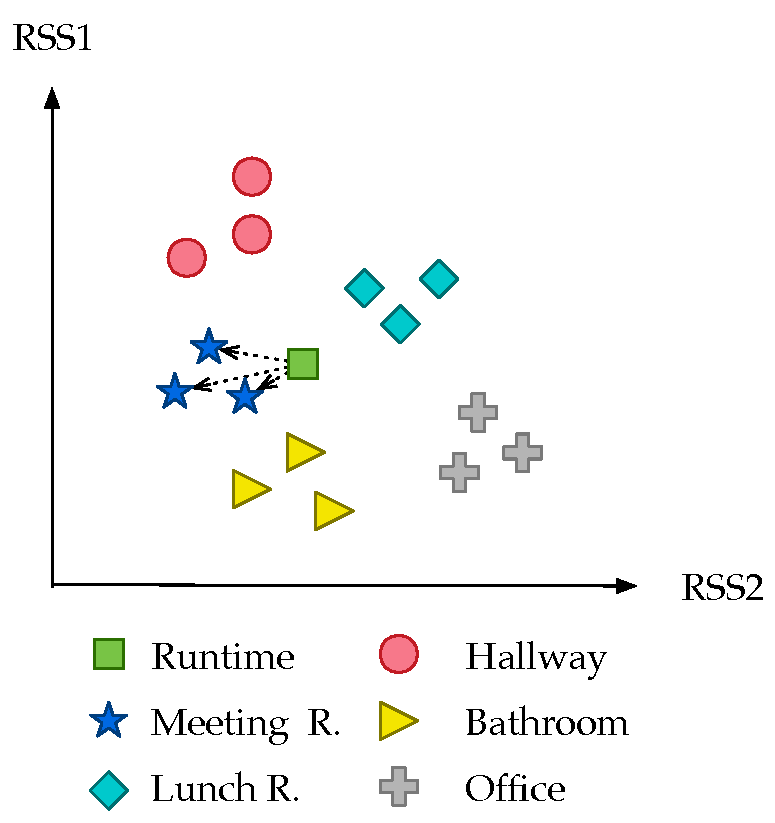
\includegraphics[scale=0.55]{KNN.pdf}
\caption[Example of KNN classification of a position between the target sub-areas]{Example of KNN classification of the current position between the target sub-areas. For each room, three signal scans have been performed. The classification assigns the most likely position based on a majority vote with $K=3$.}
\label{fig:KNN}
\end{figure}

\item \textbf{Bayesian method}: A Bayesian network containing the points of interest is built during the training phase. In the next step the system is trained a certain time on each of the points of interest, collecting RSS samples periodically. During the training phase, a priori probability $p(L)$ is constructed as a function of location L. Then, conditioned posteriori probabilities $p(E|L)$ are defined as the function of perceived RSS from a reference nodes in a certain location, and a given event or locations history (E). These methods are able to model impossible transitions from one location to another, in similar way as in Hidden Markov Model (HMM).

\item \textbf{Support Vector Machines (SVM)}: This method is a paradigm of Neural Networks, in which measure/observation vectors are processed. Processing is done by using a hypothesis space of linear functions over a space with a greater dimension (space of high-dimensional features) where the dimension of observations is induced by a kernel function with the purpose to obtain a hyperplane that separates linearly the observations and let to locate points in the most reliable as possible way. An hyperplane separates the set of training points into two subsets, each one containing a different label. From all possible planes there is only one optimal separating hyperplane (OSH) which is calculated by maximizing the distance between the optimal separation hyperplane and the closest training pattern, i.e. the maximum margin.

\item \textbf{Neural Networks Methods (NN)}: this method uses a Neural Network to estimate the location processing distinct RSS emitted from fixed receptor-emitters. The NN is implemented by a multilayer perceptron in which the input entries may be the RSS of each fixed receptor-emitters, and the output is likely to be in each of the locations.

\end{itemize}


\subsection{WiFi protocol}
The midrange wireless local area network (WLAN) standard, operating in the 2.4GHz Industrial, Scientific and Medical (ISM) band, has become very popular in public hot-spots and enterprise locations during the last few years. With a typical gross bit rate of 11, 54, or 108 Mbps and a range of 50-100 m, IEEE 802.11 is currently the dominant local wireless networking standard. It is, therefore, appealing to use an existing WLAN infrastructure for indoor location as well, by adding a location server. The accuracy of typical WLAN positioning systems using RSS is approximately 3 to 10 m, with an update rate in the range of few seconds.

All the functionality of the protocol is reflected in the packet headers. RF technology and station mobility impose some complex requirements on 802.11 WLAN networks. This added complexity is reflected in the long physical layer convergence protocol (PLCP) headers as well as the data-rich MAC header. The packet compared with the Ethernet structure is showed in figure \ref{fig:802}.

\begin{figure}[h!tb]
\centering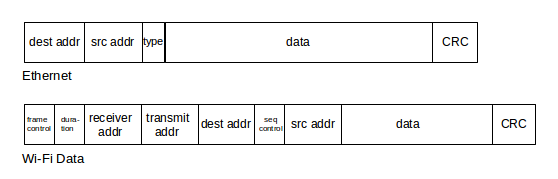
\includegraphics[scale=0.8]{802.png}
\caption{}
\label{fig:802}
\end{figure}

\subsection{Bluetooth protocol}
Bluetooth is a wireless technology standard for exchanging data over short distances (using short-wavelength UHF radio waves in the ISM band from 2.4 to 2.485 GHz) from fixed and mobile devices, and building personal area networks.
Nowadays, various mobile devices (most of commercially available phones, personal digital assistants, etc.) are equipped with Bluetooth radio transceivers. Due to its broad adoption, Bluetooth can be considered a highly ubiquitous standard. Bluetooth was originally a codename for a project lead by a Special Interest Group (SIG) consisting of major companies, like Ericsson, Intel and Nokia. The Bluetooth bit rate is lower (1 Mbps), and the range is shorter (typically
10-15 m) with respect to Wi-Fi. Moreover, Bluetooth is a lighter standard and supports several other networking services in addition to IP. For positioning, it is suggested to employ received signal strength indications (RSSI), since RSSI decreases with distance between sender and receiver. Since Bluetooth is a low-cost and low-power technology (Bluetooth tags are small size transceivers), it can be intended as an efficient solution to design IPSs. The Bluetooth positioning systems suffer from the same drawbacks of RF positioning technique in complex and full of obstacles indoor situations.


\subsubsection{Bluetooth 4.0 or Bluetooth Low Energy (BLE)}
\label{subsec:BLEprotocol}

Bluetooth v4.0 introduced Bluetooth Low Energy in 2014, officially known as BLE or Bluetooth Smart. This specification introduced a completely different wireless radio that was smaller, cheaper and lower power to meet the needs of these new applications. The wide support for it in smartphones, tablets and embedded systems makes BLE one of the most appealing protocol for the Internet of Things communications.

\smallskip
BLE specification divides Bluetooth devices in two classes: \emph{Central} and \emph{Peripheral} devices. Central devices can scan for other devices and initiate a communication. Usually, the central is a smartphone, tablet or a PC.
Peripheral wait for connections or broadcast unconnected signals coming from sensors. Typically, the slave is a small device like a fitness tracker or a smart-watch that wait for a central device and broadcast the sensed data.
Another type of peripheral device is the Bluetooth beacon, a small devices usually battery powered that continuously broadcast a unique identifier in the surrounding area for ranging applications. Some examples of BLE beacons on the market are the Estimote beacon or the Apple iBeacon.

BLE has two ways of communicating. The first way to communicate is to receive packets using a \emph{Connection}, where both the peripheral and central send packets.
The second way is using \emph{Advertisements}, where a BLE peripheral device broadcasts packets to every device around it. The receiving device can then act on this information or connect to receive more information.
Advertising is by design unidirectional. A Central device can't send any data to the Peripheral device without a connection. But a single peripheral can advertise to multiple masters in the area.

\subsubsection{Apple iBeacon protocol}
\label{subsec:ibeacon}
The iBeacon protocol, since the release of iOS 7, allows a Apple devices to receive push notifications when users enter (or exit) in (from) a iBeacon region. In addition, iOS applications can also evaluate the relative distance among the iBeacons. In iOS, regions associated with an application are continuously tracked, including when the application itself is not running; if a region boundary is crossed, the application is activated in background to handle the event. A possible application of iBeacon is a store where users receive a welcome (plus, eventually, a set of special offers) whenever they enter the store. Usually, in this kind of applications, the accuracy in determining the location of the users is not critical, and even an approximation of several meters can be acceptable.

\subsection{Existing Wireless IPS}
\label{subsec:wips_soa}

In this section the most relevant wireless indoor positioning exploiting WiFi and Bluetooth are reported.

\subsubsection{WiFi IPS}
\label{subsubsec:wifi_soa}

ARIEL \cite{Jiang2012} is a fully automated indoor room localization system. To accurately identify rooms without extensive manual annotation, they developed a number of novel techniques. First, a zone-based clustering algorithm that accurately identifies room occupancy hotspot(s) using Wi-Fi signatures. A clustering algorithm based on motion to identify inter-zone correlation, thereby distinguishing different rooms. An energy efficient motion detection algorithm to minimize the noise of Wi-Fi fingerprints.\\
ARIEL has been implemented and deployed for a 10-month study with 21 participants. The evaluation results demonstrate that their automated clustering algorithm generates clusters that are high representative of individual rooms and achieves high accuracy (95\%) for room localization. The accuracy is comparable to existing techniques that require manual annotation.

Beder and Klepal \cite{Beder2012} focused on the likelihood observation function used in fingerprinting based localization. They proposed two improvements on the commonly used Gaussian approach directly addressing two well-known issues. The first issue was the differing antenna attenuation between different devices, that they addressed by explicitly estimating a global offset thereby considering only relative differences between vectors of received signal strength measurements. The second issue was dealing with environments where not every beacon is visible everywhere, which they proposed to address by explicitly modeling the pickup probability of beacons using Gibbs distributions. Both improvements of the likelihood observation function were shown to increase the performance of their localization system. A suitable distance metric between signal strength measurements is at the core of every fingerprinting based localization system, however their findings are likely to improve all systems currently relying on a purely Gaussian approach.\\
during the 2014 Microsoft Indoor Localization Competition, 22 different solutions to indoor localization from different teams around the world were put to test in the same unfamiliar space, and the system deployed by Beder and Klepal \cite{Beder2012} performed better in the infrastructure-free (WiFi) category.


\subsubsection{Bluetooth IPS}
\label{subsubsec:bt_soa}

Zhu et al. \cite{Zhu2014} proposed one of the most relevant RSSI based Bluetooth positioning method. As usual, there are two phases in their positioning procedure: offline training and online locating. In the phase of offline training, they used piecewise fitting based on the log-normal distribution model to train the propagation model of RSSI for every BLE reference node. They design a Gaussian filter to pre-process the receiving signals in different sampling points. In the phase of online locating, they used weighted sliding window to reduce fluctuations of the real-time signals. In order to reduce the errors of targets coordinates caused by ordinary least squares method, they propose a collaborative localization algorithm based on Taylor series expansion. Another feature of their method is the active learning ability of BLE reference nodes.\\
Every reference node adjusts its pre-trained model according to the received signals from detecting nodes actively and periodically, which improve the accuracy of positioning. Experiments showed that the probability of locating error less than 1.5 meter is higher than 80\%using their positioning method.

Nacci et al. \cite{Conte2014} proposed BlueSentinel, a Bluetooth Low Energy occupancy detection system based on the Apple iBeacon protocol, with the aim to provide an energy efficient solution. In particular they proposed a modification of the iBeacon protocol, still based on BLE, in order to overcome the limitation that allows mobile devices to detect iBeacons only when entering and exiting from beacons proximity. The main idea of their implementation was to change the way the beacons advertise the region associated with them. Instead of correlate each one of them with only a single region, they let the beacons advertise more than one region, in a cyclic sequence. Thanks to this, they was able to create false events that force the operating system to wake up the mobile application more frequently.\\
The application was in charge of computing the position using RSS values and transmitting the location data to the BMS through HTTP requests.\\
The results confirmed that HTTP protocol over WiFi, even if simple to use, is not the best choice when a continuous communication is required. A test performed on a Android device (using HTTP over WiFi) showed that the battery discharged completely in only 4 hours. A different test showed that the energy consumption related to BLE tasks was \numrange{5}{10}\% of the consumption related to WiFI. This demonstrates that true low power state was guaranteed only for the stationary device (beacon) while the mobile device was forced to heavily affect the battery, increasing users effort and intrusiveness. Some consideration on this issue are reported in the next section (\ref{subsec:wips_od}).

\subsection{Indoor Localization for Occupancy Monitoring}
\label{subsec:wips_od}
The problem of monitoring the occupants location in smart buildings can be erroneously considered equal to the more traditional indoor localization problem. Although the same localization algorithms and techniques can be applied, their implementations requires relevant structural differences.

\smallskip
The main purpose of traditional indoor localization systems is to provide to the user its position on the building. The location information is exploited for navigation apps that assist the user moving from a starting point to a destination in the building, or more generally to orient the user in the indoor environment. At this purpose, signal analysis and localization algorithms are always executed on the mobile device.
Scans for wireless signals and location computation usually involve high battery consumption for the mobile devices. However, the mobile energy efficiency is not taken in consideration by the majority of the existing wireless IPS because orientation and navigation tasks are usually executed by users for a limited execution time (typically few minutes) and don't affect the battery lifetime.

\smallskip
Occupancy monitoring for smart buildings shows requirements extremely different. First, the main purpose is to obtain users presence and position information at the infrastructure level, the so called Building Management System (BMS). Here the occupancy information can be exploited to regulate automatic systems (e.g. HVAC and lighting), build occupancy probability profiles, expose occupancy information to safety applications, and so on.
Since the information is required in real-time on the infrastructure side (back-end), traditional indoor positioning systems that compute location on mobile device needs to transfer the location data through mobile connectivity.

Take in consideration WiFi based IPS as shown in figure \ref{fig:wfips_od}. The mobile device compute its position exploiting signals coming from WiFi access points. In order to monitor its position in real-time, the mobile application needs to upload the current position continuously, generating an interminable connection with high energy consumption (red connection in fig.~\ref{fig:wfips_od}). Since occupancy monitoring is required to work potentially for many hours of the day, the approach become unsustainable for the mobile battery. In addition, an energy-hungry application is intrusive for the user point of view and less likely to be adopted for continuous monitoring.


\begin{figure*}
\center
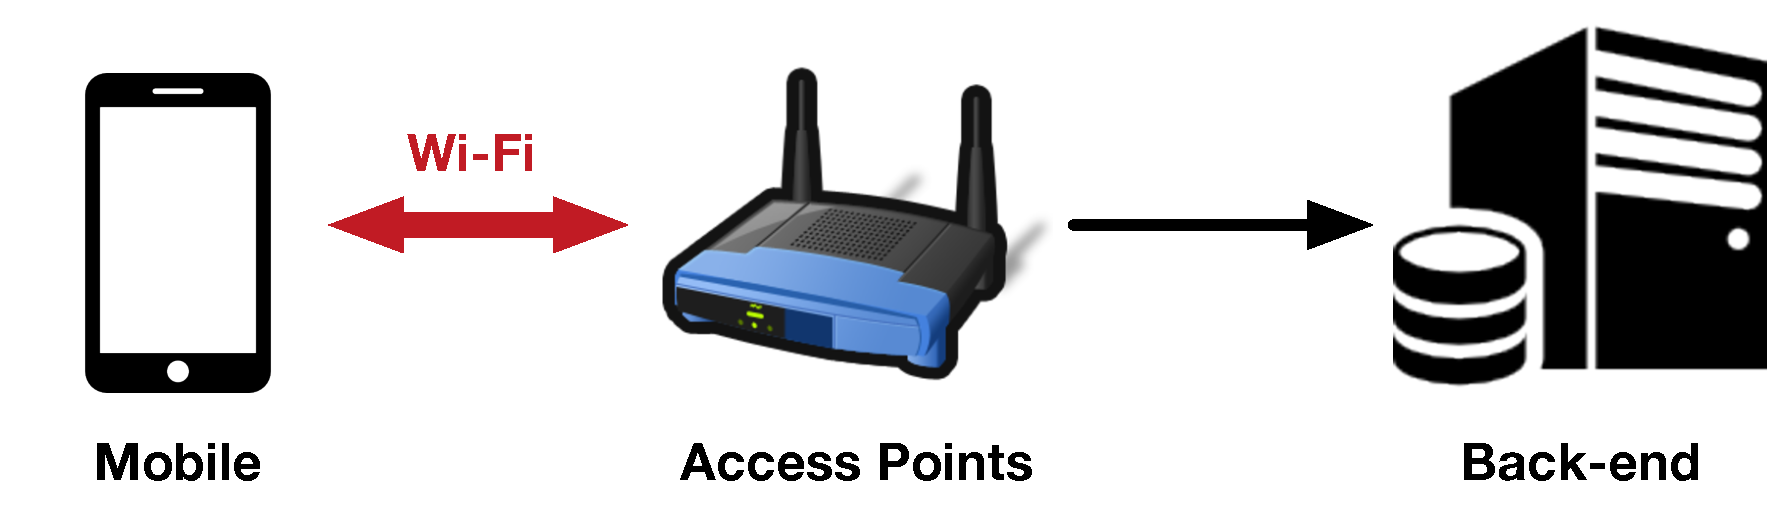
\includegraphics[scale=0.3]{protocololdwf.pdf}
\caption{Common WiFi based IPS applied for real-time occupancy monitoring.}\label{fig:wfips_od}
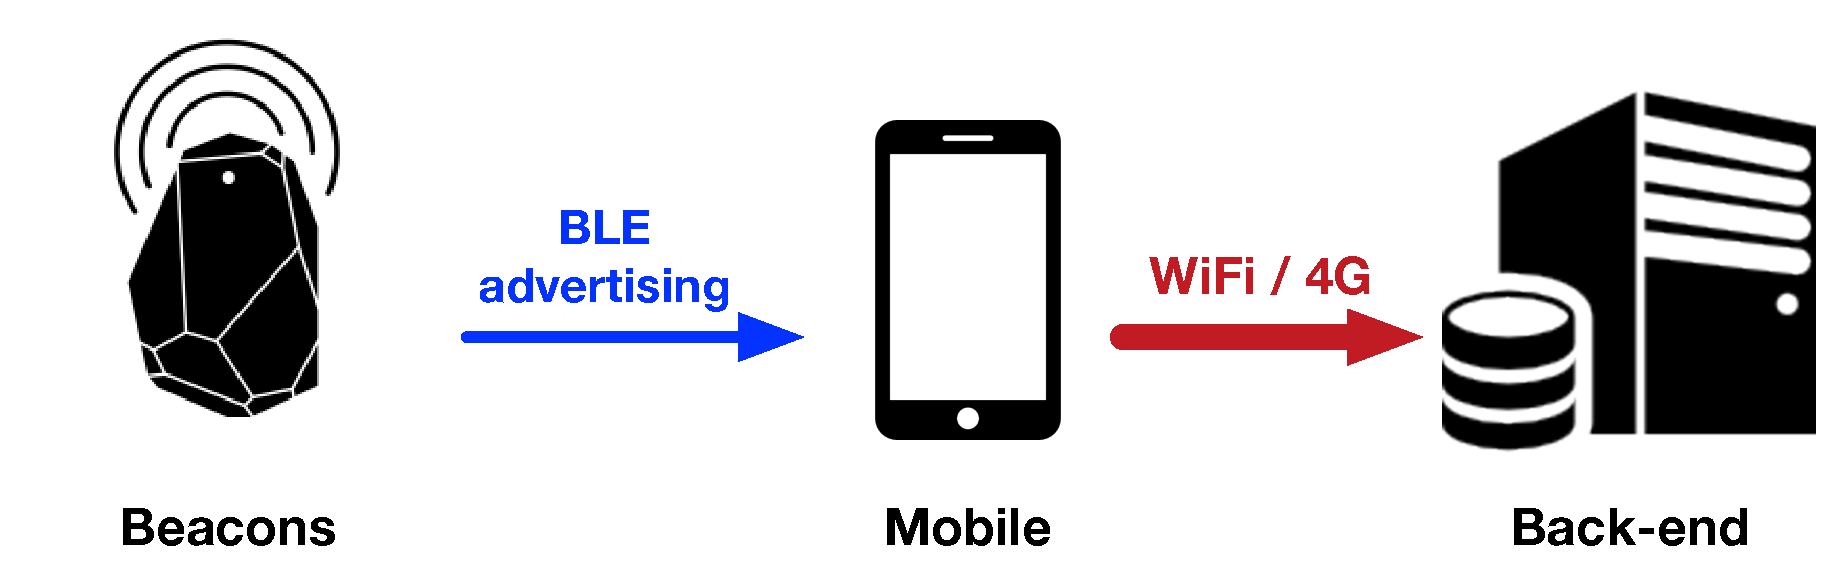
\includegraphics[scale=0.3]{protocololdbt.pdf}
\caption{Common Bluetooth based IPS applied for real-time occupancy monitoring.}\label{fig:btips_od}
\end{figure*}

In case of Bluetooth Low Energy, the employment of reference nodes such as beacons enable to provide users with their location using a low power communication. The wide popularity of the Apple iBeacon or the Estimote in commercial contexts have proved that BLE beacons are a suitable technology for providing users ranging applications and location aware services. However, in the context of location monitoring, they show the same limitations of WiFi based systems, as reported in figure \ref{fig:btips_od}. In order to retrieve position in real-time at the BMS level, the device needs to send its current position continuously through mobile connectivity, generating a long connection characterized by high energy consumptions.

% separate figures
% \begin{figure}[h!tb]
% \centering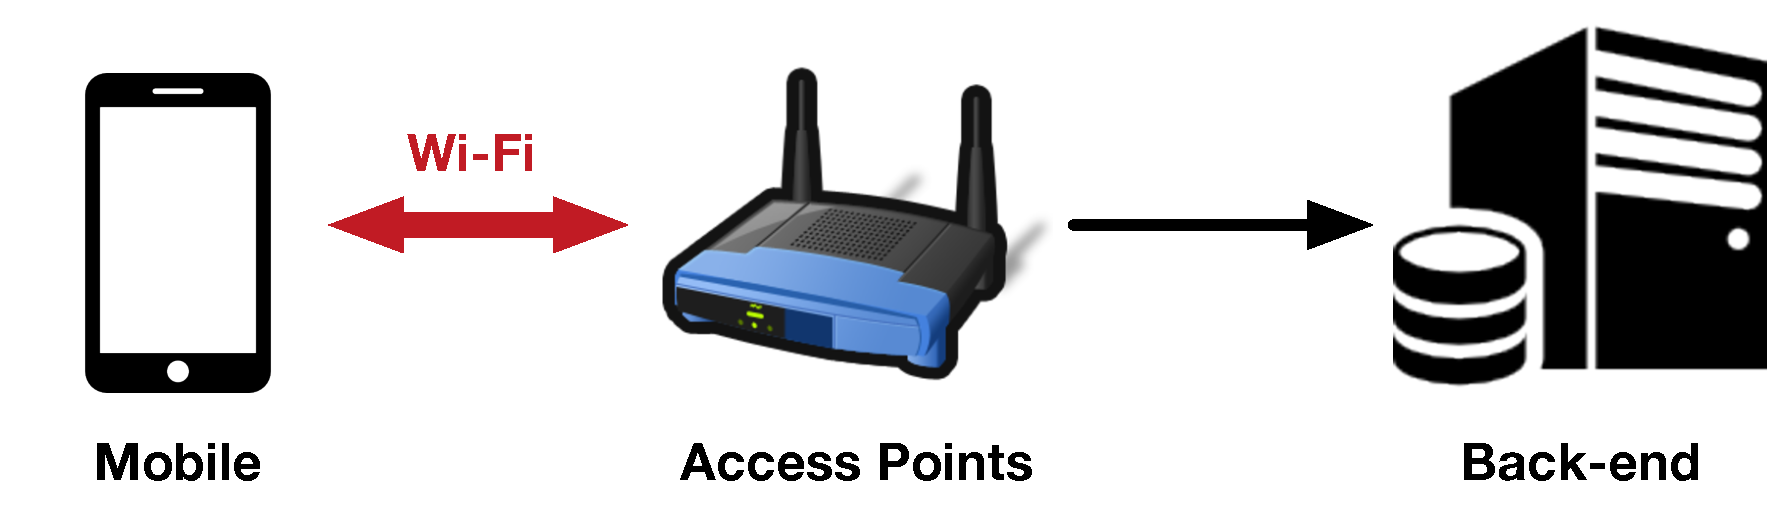
\includegraphics[scale=0.8]{protocololdwf.pdf}
% \caption{}
% \label{fig:wfips_od}
% \end{figure}\begin{figure}[h!tb]
% \centering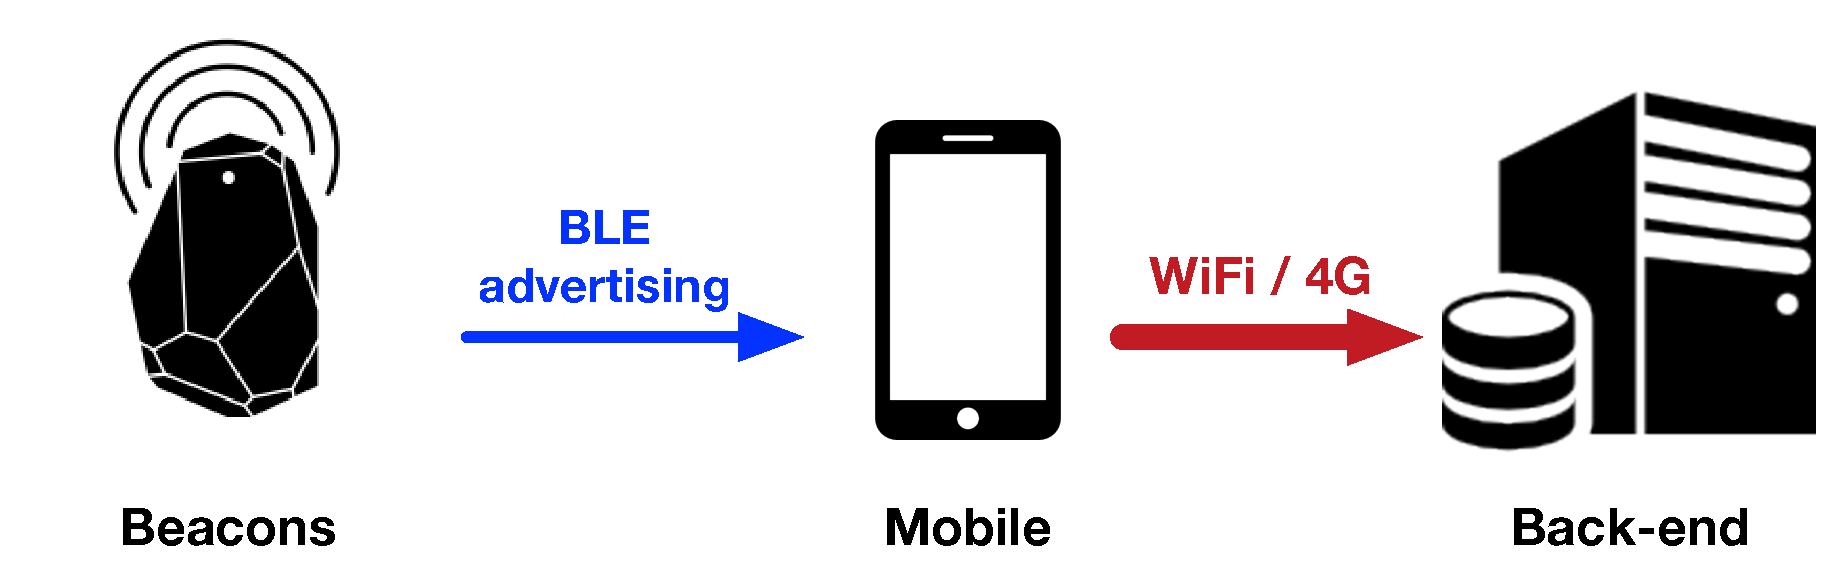
\includegraphics[scale=0.8]{protocololdbt.pdf}
% \caption{}
% \label{fig:btips_od}
% \end{figure}

\section{Comparison}
\label{sec:comparison}

In this last section, all the occupancy detection monitoring systems from existing literature that have been illustrated during this chapter are summarized and compared in table~\ref{tab:od_soa}. Extra devices for building refers to any hardware installation required in common buildings such as offices or schools. WiFi hotspots are considered already present appliances in the building infrastructure. Installation complexity, as defined by Akkaya et al. in \cite{Akkaya2015}, is represented by three tiers from low to high complexity. User intrusiveness is an indicator of how much the its activity is negatively affected by the system. When battery consumption is high, user intrusiveness is also considered high.\\
Accuracy has been considered high if the system was able to localize a user within circumscribed area with an accuracy greater than 85\%. 
%
% ------------------------------------------------------------------------ %
%
\begin{sidewaystable}
%
\caption[Comparison between the most relevant Occupancy Monitoring systems in literature.]{Comparison between the most relevant Occupancy Monitoring systems in literature.}
%
\label{tab:od_soa}
%
\centering
%
\renewcommand{\arraystretch}{0.65}
%
\begin{tabulary}{\textheight}{>{\bfseries}L L L L L L L L L L}
%
\toprule
%
\textbf{Approach} &
	\textbf{Technology}	& \textbf{Extra devices building side}	 & \textbf{Installation complexity}
	& \textbf{Extra device user side} & \textbf{Mobile consumption} & \textbf{User intrusiveness}
	& \textbf{High accuracy} & \textbf{Real-time detection} & \textbf{User identification}\\ 
%
\midrule
%
\cite{Melfi2011}  	& Implicit network sensing & No & Tier \rom{1} & No & None & Very Low & No & No & No\\
%
\cite{Balaji2013}  	& Implicit network sensing & No & Tier \rom{1} & No & None & Very Low & No & No & Yes\\
%
\midrule
%
\cite{Beltran2013}  & Ambient sensors & Yes	& Tier \rom{3} & No & None & Low & No & No & No\\
%
\cite{Cossio2012}   & Ambient sensors & Yes	& Tier \rom{3} & No & None & Low & No & No & No\\
%
\midrule
%
\cite{Erickson2013} & Cameras & Yes	& Tier \rom{2} & No	& None & High & Yes & Yes & No\\
%
\midrule
%
\cite{Jiang2012}  	& WiFi localization	& No & Tier \rom{2} & Yes & High & High & Yes & Yes & Yes\\
%
\cite{Beder2012}  	& WiFi localization	& No & Tier \rom{2} & Yes & High & High & Yes & Yes & Yes\\
%
\cite{Zhu2014}  	& Bluetooth localization & Yes & Tier \rom{2} & Yes & High & High & Yes & Yes & Yes\\
%
\cite{Conte2014}  	& Bluetooth localization & Yes & Tier \rom{2} & Yes	& High & High & Yes & Yes & Yes\\
%
\midrule
%
Proposed approach 	& BLE sensor network & Yes & Tier \rom{2} & Yes & Low & Low & Yes & Yes & Yes\\
%
\bottomrule 
%
\end{tabulary}
%
\end{sidewaystable}



\pagebreak

% Solutions based on wireless technologies have obtained the best results in terms of accuracy, spacial and temporal resolution. They usually make use of common Wi-Fi access points to locate the user's device inside the building.\\
% The most commons approaches use trilateration (Fig~\ref{fig:trilater}), triangulation and time-of-flight techniques. Although these are consolidate and performant techniques in localization (such as GPS systems), they have the drawback to require the exact position of each AP inside the building: the entire floor plan must be measured, as well as the distances between all access points, causing hard and long installations.\\
% In addition, the constant exchange of packets via WiFi is characterized by medium/high power consumption levels, so an employment for many hours of the day can be considered not sustainable for the mobile devices battery and too many intrusive for the user.\\
% An alternative to the WiFi access points are Bluetooth Low Energy (BLE) beacons. A beacon is a small wireless device that constantly broadcasts radio signals to nearby smartphones. This transmission is called \emph{advertising}, and each device advertise a universally unique identifier (UUID). In this way, mobile apps can listen for that signal and, when they receive it, trigger the correct location-based action.